\setAuthor{Koit Timpmann}
\setRound{lõppvoor}
\setYear{2006}
\setNumber{G 1}
\setDifficulty{1}
\setTopic{Elektriahelad}

\prob{Mõõteriistad}
Vooluringis on ampermeeter ja voltmeeter ühendatud jadamisi. Klemmidele on rakendatud pinge $U = \SI{9}{V}$. Kui voltmeetriga ühendada rööbiti takisti $R$, väheneb voltmeetri näit kaks korda, ampermeetri näit aga suureneb kaks korda. Kui suurt pinget näitas voltmeeter enne ja pärast takisti ühendamist?

\begin{center}
	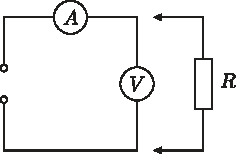
\includegraphics[width=0.5\linewidth]{2006-v3g-01-yl}
\end{center}

\hint
Ampermeetri ja voltmeetri pingete summa peab olema võrdne klemmidele rakendatava pingega nii enne kui ka pärast takisti ühendamist.

\solu
Olgu alguses ampermeetri ja voltmeetri pinged vastavalt $U_A$ ja $U_V$. Jadaühenduse korral kehtib
\[
U_A + U_V = \SI{9}{V}.
\]
Pärast takisti lisamist suurenes ampermeetrit läbiv vool ja seega ka pinge kaks korda. Teisisõnu, ampermeetri uus pinge oli $2U_A$. Pinge voltmeetril aga vähenes kaks korda ja oli $\num{0,5}U_V$. Kirchhoffi pinge seaduse kohaselt
\[
2U_A + \num{0,5}U_V = \SI{9}{V}.
\]
Lahendades kahest võrrandist koosneva võrrandisüsteemi, saame $U_A = \SI{3}{V}$ ja $U_V = \SI{6}{V}$. Seega voltmeetril pinge oli alguses \SI{6}{V} ning lõpus \SI{3}{V}.
\probend